\documentclass{article}

\usepackage[utf8]{inputenc}
\usepackage[english]{babel}
\usepackage{graphicx}
\usepackage{listings}
\usepackage{xcolor}                 % Define custom colour and use using \textcolor{colour}{text}
\usepackage{float}

\usepackage{rotating}               % 90 degrees image
\usepackage{lscape}                 % landscape 

\usepackage{hyperref}

\usepackage{longtable}              % Predefined width table
\usepackage{csquotes}               % Use proper \enquote{quotations}
\usepackage{bytefield}              % Beautiful register figures 
\usepackage[block=ragged,alldates=comp,backend=biber]{biblatex} % Reference management

\definecolor{celadon}{rgb}{0.67, 0.88, 0.69}
\newcommand{\colorbitbox}[3]{%
\rlap{\bitbox{#2}{\color{#1}\rule{\width}{\height}}}%
\bitbox{#2}{#3}}

\usepackage{tikz}
\usepackage{tikz-qtree}

%\bibliographystyle{IEEEtran}
\bibliography{references.bib}

\usepackage%
[%
left=2cm,% left margin
right=2cm,% right margin
top=3cm, % top margin
bottom=3cm,% bottom margin
a4paper% other options: a0paper, a1paper, a2paper, a3paper, a4paper, a5paper, a6paper, and many more.
]{geometry}

\usepackage{pbox}

\title{DLLGraph}
\author{Youri Klaassens, Nathan Godefroij}
\date{October 2019}

\definecolor{mGreen}{rgb}{0,0.6,0}
\definecolor{mGray}{rgb}{0.5,0.5,0.5}
\definecolor{mPurple}{rgb}{0.58,0,0.82}
\definecolor{backgroundColour}{rgb}{0.95,0.95,0.92}

\setlength{\parindent}{0pt}

\lstdefinestyle{CStyle}{
    backgroundcolor=\color{backgroundColour},   
    commentstyle=\color{mGreen},
    keywordstyle=\color{magenta},
    numberstyle=\tiny\color{mGray},
    stringstyle=\color{mPurple},
    basicstyle=\footnotesize,
    breakatwhitespace=false,         
    breaklines=true,                 
    captionpos=b,                    
    keepspaces=true,                 
    numbers=left,                    
    numbersep=5pt,                  
    showspaces=false,                
    showstringspaces=false,
    showtabs=false,                  
    tabsize=2,
    language=C
}

\tikzset{every tree node/.style={minimum width=2em,draw,circle},
         blank/.style={draw=none},
         edge from parent/.style=
         {draw, edge from parent path={(\tikzparentnode) -- (\tikzchildnode)}},
         level distance=1.5cm}

\lstdefinestyle{ValgrindStyle}{
    backgroundcolor=\color{backgroundColour},   
    breakatwhitespace=false,         
    breaklines=true,                 
    captionpos=b,                    
    keepspaces=true,                 
    numbers=left,                    
    numbersep=5pt,                  
    showspaces=false,                
    showstringspaces=false,
    showtabs=false,                  
    tabsize=2,
    language=C
}

\addbibresource{references.bib}
\begin{document}

\begin{titlepage}
	\centering
	\smallbreak                         % smallbreak, medbreak, bigbreak
	\rule{\linewidth}{0.2 mm} \\[0.4 cm]
	{\huge \bfseries Basic Real-Time Operating System}\\
	\smallbreak
	\par{\large targeting the ARMv7-M architecture}      
	\rule{\linewidth}{0.2 mm} \\[1.5 cm]
	\vspace*{0.5 cm}
	\par{\LARGE \textit{ROS01}, Rotterdam \today }\\[1.0 cm]
    
\includegraphics[scale=0.99]{img/HR.png}\\[1.0 cm]	

	


\begin{figure}[!b]
	\begin{minipage}{0.5\textwidth}
		\begin{flushleft} \large
			\emph{Student:}\\
		    Nick van Endhoven\\
            0998831hr.nl\\
            Breda\\
			\end{flushleft}
			\end{minipage}~
			\begin{minipage}{0.5\textwidth}
 
		\begin{flushright} \large
            \emph{Student:}\\
			Youri Klaassens\\
            0996211@hr.nl\\
            Zwaag\\
		\end{flushright}
        
	\end{minipage}\\[2 cm]
\end{figure}
    
    
    
    
	
\end{titlepage}


\tableofcontents
\thispagestyle{empty}

\newpage

\pagenumbering{arabic}
\setcounter{page}{1}

\section*{Version history}
\addcontentsline{toc}{section}{Version history}

\definecolor{darkpink}{rgb}{1.0, 0.13, 0.32}

\begin{longtable}{| p{.08\textwidth} | p{.12\textwidth} | p{.38\textwidth} | p{.30\textwidth} |}

    \hline
    \textcolor{darkpink}{Version} & \textcolor{darkpink}{Date} & \textcolor{darkpink}{Change(s)} & \textcolor{darkpink}{Note} \\
     
    \hline
    \textbf{0.1} & 11-30-2019 & Initial document & Created version history, introduction, acknowledgement and appendix. \\

    \hline

    \textbf{0.2} & 12-07-2019 & Minor changes in Appendix \ref{subsec:appendix_delay} & Documented the first assignment (toggling LEDs) \\

    \hline

    \caption{Overview of the different versions}
    \label{tab:version}

\end{longtable}


\newpage
\section{Introduction}

For the Real-time Operating Systems course (ROS01) taught at Rotterdam University of Applied Science,
the authors had to implement a scheduler for a Real-time Operating System developed by one lecturers.
Because these types of programming issues like implementing a scheduler require the programmer to be able to program at a low level and it cannot be assumed that every student following this course is familiar with low level progamming (both in the C programming language and assembler), this course contains multiple assingments to bridge this gap.
The code has been flashed and tested on the CC3220s development board (Figure \ref{fig:cc3220s}). The compiler used is TI v18.12.2.LTS.

What's worth mentioning is that some code snippets in this document make a function call to \texttt{delay\_1sec()}.
Because this is used quite a few times and redundant to have multiple definitions in this document its implementation can be seen in Appendix \ref{subsec:appendix_delay}.


\begin{figure}[H]
    \centering

    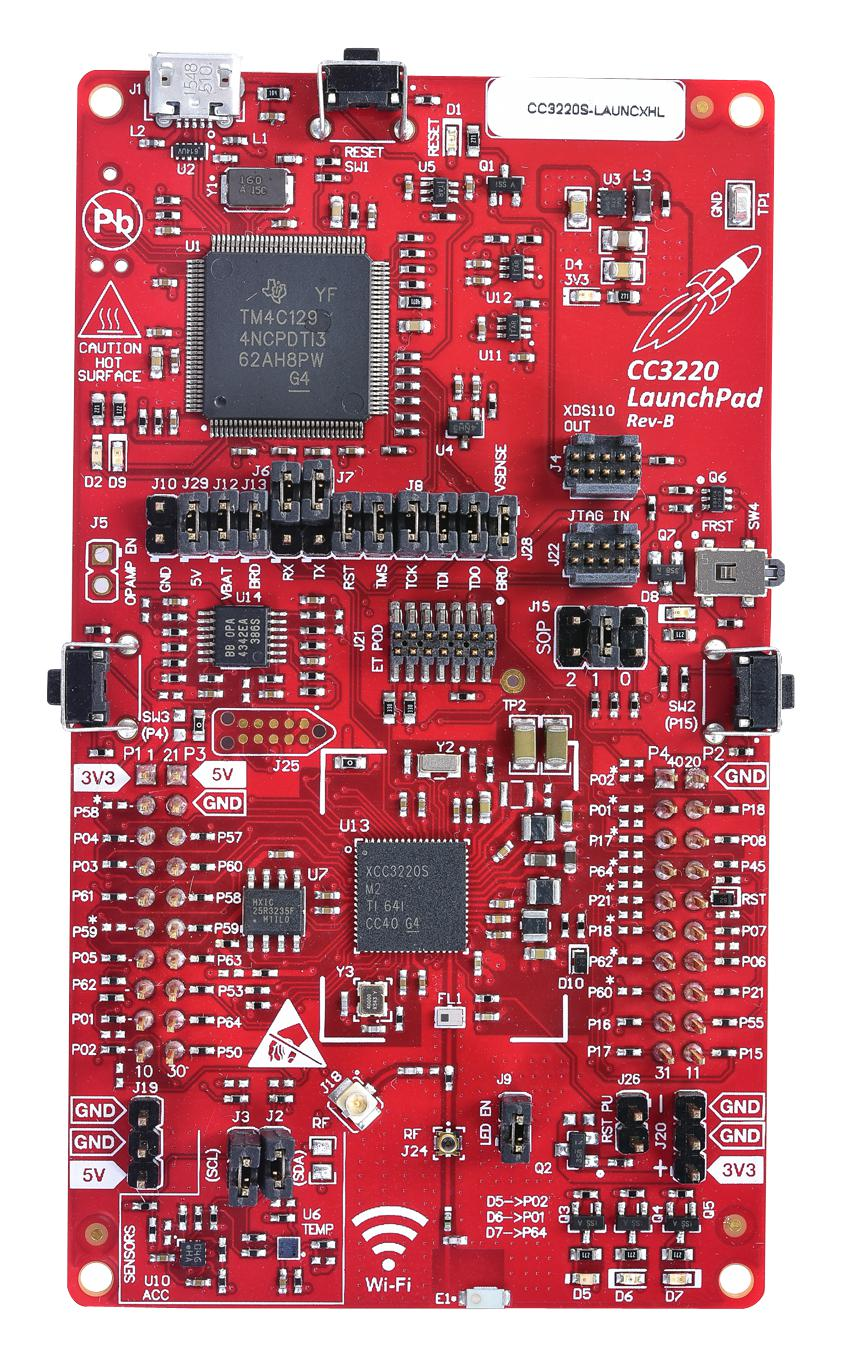
\includegraphics[angle=90,scale=0.2]{img/cc3220s.jpg}

    \caption{The CC3220s development board used during labs}
    \label{fig:cc3220s}

\end{figure}


\section{Toggling LEDs bottom-up}

The purpose of the first assignment is to become familiar with low level programming.
This is done by toggling LEDs using different levels of abstraction.
The sequence of this \enquote{LED show} can be seen in Table \ref{tab:led_scheme}.
Between every sequence should be a delay of approximately 1 second.

\begin{table}[H]
    \centering
    \begin{tabular}{|c|c|c|}
        \hline
        \textcolor{darkpink}{\textit{Green}} & \textcolor{darkpink}{\textit{Yellow}} & \textcolor{darkpink}{\textit{Red}}\\
        \hline
        0 & 0 & 0 \\
        \hline
        0 & 0 & 1 \\
        \hline
        0 & 1 & 0 \\
        \hline
        0 & 1 & 1 \\
        \hline
        1 & 0 & 0 \\
        \hline
        1 & 0 & 1 \\
        \hline
        1 & 1 & 0 \\
        \hline
        1 & 1 & 1 \\
        \hline
    \end{tabular}
        
    \label{tab:led_scheme}
    \caption{Order of visualisation of different LEDs}
\end{table}

As said earlier, these \enquote{LED show} should be programmed on three different levels of abstraction.
The first one is no abstraction at all using a programming technique called Direct Register Manipulation (DRM) \cite{IntroEmbeddedSystems}.
The second implementation should make use Driverlib.
The third implementation should make use of the Texas Instruments (TI) Driver.

\newpage
\subsection{Direct Register Manipulation}

Listing \ref{lst:led_drm} shows the source code to toggle LEDs according to Table \ref{tab:led_scheme}.
The reader may wonder why the implementation of \texttt{delay\_1sec()} is missing. 
This is because it is a common function used in lots of code snippets throughout this document.
For the implementation details see Appendix \ref{subsec:appendix_delay}.
Now follows an explanation about interesting lines of code.
Line \ref{line:drm_arcm} enables the GPIOA peripheral during run mode (see Figure \ref{fig:gpio0clken}).
This program does not enter sleep mode or deep sleep mode. Setting bit 8 and bit 16 (Figure \ref{fig:gpio0clken}) does not make sense.

\begin{figure}[H]
\centering

\begin{bytefield}[endianness=big, bitwidth=3.0em]{30}
\bitheader[lsb=2]{16-31} \\
    \bitbox{15}{\tiny Reserved} &
    \colorbitbox{celadon}{1}{\tiny DSLPCLKEN} \\ [3ex]
\bitheader[lsb=-14]{0-15} \\
    \bitbox{7}{\tiny Not Used}
    \colorbitbox{celadon}{1}{\tiny SLPCLKEN}
    \bitbox{7}{\tiny Not Used}
    \colorbitbox{celadon}{1}{\tiny RUNCLKEN}
\end{bytefield}

\caption{\texttt{GPIO0CLKEN} register for the CC3220s}
\label{fig:gpio0clken}

\end{figure}

The behavior of the pins being used must be configured.
The assignment only requires the use of GPIO9, GPIO10 and GPIO11 because the built-in LEDs are routed to these pins.
Configuration for these pins are done in Line \ref{line:drm_conf9} up to and including Line \ref{line:drm_conf11}.
The value 0x60 is written to the \texttt{GPIO\_PAD\_CONFIG\_x} register where x is 9, 10 and 11.
It affects the second nibble of the register.
Since only bit 1 and bit 2 of the nibble are affected it does not set the bit in the \texttt{open drain} field (Figure \ref{fig:padconf}).
Writing $001_{2}$ to the \texttt{DRIVE STRENGTH} field means that the related GPIO pin will drive 6 mA.

\begin{figure}[H]
\centering

\begin{bytefield}[endianness=big, bitwidth=3.0em]{30}
\bitheader[lsb=2]{16-31} \\
    \bitbox{16}{\tiny Reserved} \\ [3ex]
\bitheader[lsb=-14]{0-15} \\
    \bitbox{4}{\tiny Reserved}
    \colorbitbox{celadon}{1}{\tiny over-riding buffer}
    \colorbitbox{celadon}{1}{\tiny override value}
    \colorbitbox{celadon}{1}{\tiny pulldown}
    \colorbitbox{celadon}{1}{\tiny pullup}
    \colorbitbox{celadon}{3}{\tiny DRIVE STRENGTH}
    \colorbitbox{celadon}{1}{\tiny open drain}
    \colorbitbox{celadon}{4}{\tiny CONFMODE}
\end{bytefield}

\caption{\texttt{GPIO\_PAD\_CONFIG\_x} register for the CC3220s}
\label{fig:padconf}

\end{figure}

A GPIO pin is either input or output. Writing a 1 to the \texttt{GPIO\_DIR} register (Figure \ref{fig:dirconf}) configures a GPIO pin as output pin.
Writing a 0 to the \texttt{GPIO\_DIR} register configures a GPIO pin as input pin.
Because this program only needs GPIO9, GPIO10 and GPIO11 the program needs to write a 1 to bit 1, bit 2 and bit 3 respectively.
$00001110_{2}$ is 0x0E in hexadecimal representation.
That is why the program writes 0x0E to the \texttt{GPIO\_DIR} register at Line \ref{line:drm_dir}.

\begin{figure}[H]
\centering

\begin{bytefield}[endianness=big, bitwidth=3.0em]{30}
\bitheader[lsb=2]{16-31} \\
    \bitbox{16}{\tiny Reserved} \\ [3ex]
\bitheader[lsb=-14]{0-15} \\
    \bitbox{8}{\tiny Reserved}

    \colorbitbox{celadon}{1}{\tiny DIR}
    \colorbitbox{celadon}{1}{\tiny DIR}
    \colorbitbox{celadon}{1}{\tiny DIR}
    \colorbitbox{celadon}{1}{\tiny DIR}
    \colorbitbox{celadon}{1}{\tiny DIR}
    \colorbitbox{celadon}{1}{\tiny DIR}
    \colorbitbox{celadon}{1}{\tiny DIR}
    \colorbitbox{celadon}{1}{\tiny DIR}

\end{bytefield}

\caption{\texttt{GPIO\_DIR} register for the CC3220s}
\label{fig:dirconf}

\end{figure}

Setting the output pin to logic high or logic low requires a little extra explanation.
There is a mask which should be added to the base address plus the address of the \texttt{GPIO\_DATA} register.
This prevents software from a read-modify-write operation. A change in logic level of an GPIO output pin is done in a single cycle.
The bits one would like to change should be shifted 2 positions to the right and added to base address + the \texttt{GPIO\_DATA} offset.
Line \ref{line:drm_init_data} turns the three LEDs off by writing $00000000_{2}$ or 0x00 to the \texttt{GPIO\_DATA} register.
However, because of the mask added to the address only bit 1, bit 2 and bit 3 are affected.

\begin{figure}[H]
\centering

\begin{bytefield}[endianness=big, bitwidth=3.0em]{30}
\bitheader[lsb=2]{16-31} \\
    \bitbox{16}{\tiny Reserved} \\ [3ex]
\bitheader[lsb=-14]{0-15} \\
    \bitbox{8}{\tiny Reserved}

    \colorbitbox{celadon}{1}{\tiny DATA}
    \colorbitbox{celadon}{1}{\tiny DATA}
    \colorbitbox{celadon}{1}{\tiny DATA}
    \colorbitbox{celadon}{1}{\tiny DATA}
    \colorbitbox{celadon}{1}{\tiny DATA}
    \colorbitbox{celadon}{1}{\tiny DATA}
    \colorbitbox{celadon}{1}{\tiny DATA}
    \colorbitbox{celadon}{1}{\tiny DATA}

\end{bytefield}

\caption{\texttt{GPIO\_DATA} register for the CC3220s}
\label{fig:dataconf}

\end{figure}

The following things happen in an infinite loop.
Line \ref{line:drm_toggle} in Listing \ref{lst:led_drm} write a variable \texttt{index} to \texttt{GPIO\_DATA} register.
This value is shifted 1 position to the left because the first LED is positioned at GPIO9 and not at GPIO8.
Line \ref{line:drm_modulo} increments \texttt{index}. Variable \texttt{index} can hold $0 \leq index < 16$ (although $0 \leq index < 8$ would be sufficient).
The second operand of the modulo operator does not really matter as long as it is a multiple of $2^3$.
Line \ref{line:drm_sleep} makes a call to \texttt{delay\_1sec()}. The function returns after 1 second since it is a busy-wait like implementation where the CPU just burns CPU cycles.

\begin{lstlisting}[style=CStyle, caption={Toggling LEDs according to Table \ref{tab:led_scheme} using DRM programming technique}, captionpos=b, label={lst:led_drm}, escapechar=@]
#include <stdint.h>
#include <stddef.h>
#include "register_def.h"
 
#include "inc\hw_memmap.h"
#include "inc\hw_gpio.h"
#include "inc\hw_apps_rcm.h"
#include "inc\hw_ocp_shared.h"
 
/* Function delay_1sec() used to be here */

int main(void)
{
 
    HWREG(ARCM_BASE + APPS_RCM_O_GPIO_A_CLK_GATING) = 0x01; @\label{line:drm_arcm}@
 
    HWREG(OCP_SHARED_BASE + OCP_SHARED_O_GPIO_PAD_CONFIG_9) = 0x60; @\label{line:drm_conf9}@
    HWREG(OCP_SHARED_BASE + OCP_SHARED_O_GPIO_PAD_CONFIG_10) = 0x60; @\label{line:drm_conf10}@
    HWREG(OCP_SHARED_BASE + OCP_SHARED_O_GPIO_PAD_CONFIG_11) = 0x60; @\label{line:drm_conf11}@
 
    HWREG(GPIOA1_BASE + GPIO_O_GPIO_DIR) = 0x0E;    @\label{line:drm_dir}@
    HWREG(GPIOA1_BASE + GPIO_O_GPIO_DATA + (0x0E << 2)) = 0x00; @\label{line:drm_init_data}@
 
    int index = 0;
 
    while(1)
    {
        HWREG(GPIOA1_BASE + GPIO_O_GPIO_DATA + (0x0E << 2)) = (index << 1); @\label{line:drm_toggle}@
        index = (index + 1) % 16;       @\label{line:drm_modulo}@
        delay_1sec();                   @\label{line:drm_sleep}@
    }
 
    return 0;
}
\end{lstlisting}


\newpage
\subsection{Driverlib}

Driverlib is a library which provides access to peripherals.
The advantage of this is that the programmer does not need to know base addresses and offsets in order to access special function registers.
Line \ref{line:driverlib_clk} in Listing \ref{lst:led_driverlib} enables the \texttt{GPIOA1} peripheral by enabling a clock signal to the peripheral.
Line \ref{line:driverlib_pad1} up to and including Line \ref{line:driverlib_pad3} configures the GPIO9, GPIO10 and GPIO11 pin characteristics. The pins can use now a maximum of 2 mA per pin.
Note that the function accepts a macro which contains the physical pin number instead of the logical pin number.
Line \ref{line:driverlib_dir1} up to and including Line \ref{line:driverlib_dir3} configures GPIO9, GPIO10 and GPIO11 to an output pin.
Line \ref{line:driverlib_data1} up to and including Line \ref{line:driverlib_data3} turns the three LEDs off by default.

Line \ref{line:driverlib_toggle} writes the value \texttt{switcher} to the \texttt{GPIO\_DATA} register but only \texttt{GPIO\_PIN\_1}, \texttt{GPIO\_PIN\_2} and \texttt{GPIO\_PIN\_3} (which are GPIO9, GPIO10 and GPIO11) are sensitive for this value change. 
Line \ref{line:driverlib_sleep} makes a function call to \texttt{delay\_1sec()} which will return to the caller after 1 second.

\begin{lstlisting}[style=CStyle, caption={Toggling LEDs according to Table \ref{tab:led_scheme} using Driverlib library}, captionpos=b, label={lst:led_driverlib}, escapechar=@]
#include <stdint.h>
#include <stddef.h>
#include "register_def.h"
 
#include "gpio.h"
#include "pin.h"
#include "prcm.h"
 
/* GPIO 9 is PIN_64 is (red) */
/* GPIO 10 is PIN_2 is (green) */
/* GPIO 11 is PIN_1 is (yellow) */
 
/* Function delay_1sec() used to be here */
 
int main(void)
{
    PRCMPeripheralClkEnable(PRCM_GPIOA1 ,PRCM_RUN_MODE_CLK);        @\label{line:driverlib_clk}@
 
    PinTypeGPIO(PIN_64, PIN_STRENGTH_2MA, false);   /* Red LED is push-pull */  @\label{line:driverlib_pad1}@
    PinTypeGPIO(PIN_01, PIN_STRENGTH_2MA, false);   /* Yellow LED is push-pull */ @\label{line:driverlib_pad2}@
    PinTypeGPIO(PIN_02, PIN_STRENGTH_2MA, false);   /* Green LED is push-pull */  @\label{line:driverlib_pad3}@
 
    GPIODirModeSet(GPIOA1_BASE, GPIO_PIN_2, GPIO_DIR_MODE_OUT); @\label{line:driverlib_dir1}@
    GPIODirModeSet(GPIOA1_BASE, GPIO_PIN_3, GPIO_DIR_MODE_OUT); @\label{line:driverlib_dir2}@
    GPIODirModeSet(GPIOA1_BASE, GPIO_PIN_1, GPIO_DIR_MODE_OUT); @\label{line:driverlib_dir3}@
 
    GPIOPinWrite(GPIOA1_BASE, GPIO_PIN_2, ~GPIO_PIN_2);  /* Turn yellow LED off */ @\label{line:driverlib_data1}@
    GPIOPinWrite(GPIOA1_BASE, GPIO_PIN_3, ~GPIO_PIN_3);  /* Turn green LED off */   @\label{line:driverlib_data2}@
    GPIOPinWrite(GPIOA1_BASE, GPIO_PIN_1, ~GPIO_PIN_1);  /* Turn red LED off */    @\label{line:driverlib_data3}@
 
    int switcher = 0;
 
    while(1)
    {
        GPIOPinWrite(GPIOA1_BASE, GPIO_PIN_1 | GPIO_PIN_2 | GPIO_PIN_3, switcher);  @\label{line:driverlib_toggle}@
        delay_1sec();                                                               @\label{line:driverlib_sleep}@
 
        switcher = (switcher + 1) % 16;                                             @\label{line:driverlib_inc}@
    }
}
\end{lstlisting}

\newpage
\subsection{TI Driver}

\begin{lstlisting}[style=CStyle, caption={Toggling LEDs according to Table \ref{tab:led_scheme} using TI Driver}, captionpos=b, label={lst:led_ti}, escapechar=@]
void *mainThread(void *arg0)
{
    /* Call driver init functions */
    GPIO_init();
 
    /* Configure the LED */
    GPIO_setConfig(Board_GPIO_LED0, GPIO_CFG_OUT_STD | GPIO_CFG_OUT_LOW);
    GPIO_setConfig(Board_GPIO_LED1, GPIO_CFG_OUT_STD | GPIO_CFG_OUT_LOW);
    GPIO_setConfig(Board_GPIO_LED2, GPIO_CFG_OUT_STD | GPIO_CFG_OUT_LOW);
 
    /* Turn on user LED */
    GPIO_write(Board_GPIO_LED0, Board_GPIO_LED_OFF);    /* Turn red LED off */
    GPIO_write(Board_GPIO_LED1, Board_GPIO_LED_OFF);    /* Turn yellow LED off */
    GPIO_write(Board_GPIO_LED2, Board_GPIO_LED_OFF);    /* Turn green LED off */
 
    unsigned int switcher = 0;
 
    while(1)
    {
        GPIO_write(Board_GPIO_LED0, switcher & 1);
        GPIO_write(Board_GPIO_LED1, (switcher & 2) >> 1);
        GPIO_write(Board_GPIO_LED2, (switcher & 4) >> 2);
        delay_1sec();
 
        switcher = (switcher + 1) % 8;
    }
 
 
    return (NULL);
}
\end{lstlisting}



\newpage
\section{Replace busy-wait techniques using the \texttt{SysTick} timer}

Using a busy-wait technique to delay for a certain amount of time is not efficient.
Wasting \enquote{expensive} CPU cycles should be avoided whenever possible.
This is where hardware timers comes in.
Hardware timers decrement or increment a given value at a certain frequency and generates a signal if the value reached a treshold (this could be in the form of underflow or overflow aswell as reaching a certain value where 0 is the most common one).
This chapter describes the \texttt{SysTick} hardware timer.

\subsection{\texttt{SysTick} timer and interrupt using DRM}

As mentioned in the previous section, when one uses the DRM programming technique it is important that the programmer knows the microcontroller really well.
Understanding the different Special Function Registers (SFR) related to the hardware module one wants to use is a consequence.
The three SFR related to \texttt{SysTick} are described below.

\begin{figure}[H]
\centering

\begin{bytefield}[endianness=big, bitwidth=3.0em]{30}
\bitheader[lsb=2]{16-31} \\
    \bitbox{15}{\tiny Reserved} &
    \colorbitbox{celadon}{1}{\tiny COUNT} \\ [3ex]
\bitheader[lsb=-14]{0-15} \\
    \bitbox{13}{\tiny Reserved}
    \colorbitbox{celadon}{1}{\tiny CLK\_SRC}
    \colorbitbox{celadon}{1}{\tiny INTEN}
    \colorbitbox{celadon}{1}{\tiny ENABLE}
\end{bytefield}

\caption{\texttt{STCTRL} register for the CC3220s}
\label{fig:stctrl}

\end{figure}

First, there is \texttt{STCTRL} (\texttt{SysTick} Control Register) which enables the \texttt{SysTick} features \cite{CC3220s_reference_manual}.
Bit 0 (Figure \ref{fig:stctrl}) enables the \texttt{SysTick} module if this bit is set or disables the \texttt{SysTick} module if this bit is cleared.
The \texttt{SysTick} module will generate an interrupt only if bit 1 is set.
The clock source fed into the \texttt{SysTick} module can be the system clock if bit 3 is set or a precision internal oscillator if bit 3 is cleared \cite{CC3220s_reference_manual}.


\begin{figure}[H]
\centering

\begin{bytefield}[endianness=big, bitwidth=3.0em]{30}
\bitheader[lsb=2]{16-31} \\
    \bitbox{8}{\tiny Reserved} &
    \colorbitbox{celadon}{8}{\tiny RELOAD} \\ [3ex]
\bitheader[lsb=-14]{0-15} \\
    \colorbitbox{celadon}{16}{\tiny RELOAD}
\end{bytefield}

\caption{\texttt{STRELOAD} register for the CC3220s}
\label{fig:streload}

\end{figure}

Second, there is \texttt{STRELOAD} register (Figure \ref{fig:streload}) which stores the constant that should be loaded to the \texttt{STCURRENT} register if the previous value reached value 0.
One should keep in mind that if the desired behaviour is an interrupt or a flag every $x$ ticks, one should store $x - 1$ ticks in this register.
This is because the \texttt{RELOAD} value is copied to \texttt{STCURRENT} current register if 0 is reached (so not one tick after zero).

\begin{figure}[H]
\centering

\begin{bytefield}[endianness=big, bitwidth=3.0em]{30}
\bitheader[lsb=2]{16-31} \\
    \bitbox{8}{\tiny Reserved} &
    \colorbitbox{celadon}{8}{\tiny CURRENT} \\ [3ex]
\bitheader[lsb=-14]{0-15} \\
    \colorbitbox{celadon}{16}{\tiny CURRENT}
\end{bytefield}

\caption{\texttt{STCURRENT} register for the CC3220s}
\label{fig:stcurrent}

\end{figure}

The last register is the \texttt{STCURRENT} register.
This register holds the current value being decremented.
An important detail is that the \texttt{CURRENT} field is write-clear behaviour.
This means that writing any value to this field clears the register and the \texttt{COUNT} bit of the \texttt{STCTRL} register \cite{CC3220s_reference_manual}.

\newpage
\begin{lstlisting}[style=CStyle, caption={Toggling LEDs according to Table \ref{tab:led_scheme} using DRM programming technique}, captionpos=b, label={lst:led_systick_drm}, escapechar=@]
#include <stdint.h>
#include <stddef.h>
#include "register_def.h"

#include "inc\hw_memmap.h"
#include "inc\hw_gpio.h"
#include "inc\hw_apps_rcm.h"
#include "inc\hw_ocp_shared.h"

static volatile _Bool flag_led_update;  @\label{line:drm_systick_flag}@

void SysTickHandler()   @\label{line:drm_systick_irq}@
{
    static int tick_count = 0;
    flag_led_update = tick_count == 1000 ? 1 : 0;   @\label{line:drm_systick_set_flag}@
    tick_count = (tick_count+1) % (1000 + 1);       @\label{line:drm_systick_inc}@
}

int main(void)
{

    /* Init SysTick */
    HWREG(NVIC_ST_CTRL) = 0x00;         // Disable SysTick during setup     @\label{line:drm_systick_disable}@
    HWREG(NVIC_ST_RELOAD) = 79999;      // Get every millisecond an interrupt (80 000 - 1)  @\label{line:drm_systick_reload}@
    HWREG(NVIC_ST_CURRENT) = 0x00;      // Clear any flags and set current value to 0       @\label{line:drm_systick_current}@
    HWREG(NVIC_ST_CTRL) = 0x07;         // Enable SysTick, Enable interrupt, CLK_SRC = System clock @\label{line:drm_systick_enabe}@

    /* Init LEDS */
    HWREG(ARCM_BASE + APPS_RCM_O_GPIO_A_CLK_GATING) = 0x01;     @\label{line:drm_systick_gpio_enable}@

    HWREG(OCP_SHARED_BASE + OCP_SHARED_O_GPIO_PAD_CONFIG_9) = 0x60; @\label{line:drm_systick_pad_one}@
    HWREG(OCP_SHARED_BASE + OCP_SHARED_O_GPIO_PAD_CONFIG_10) = 0x60;
    HWREG(OCP_SHARED_BASE + OCP_SHARED_O_GPIO_PAD_CONFIG_11) = 0x60;@\label{line:drm_systick_pad_three}@

    HWREG(GPIOA1_BASE + GPIO_O_GPIO_DIR) = 0x0E;            @\label{line:drm_systick_dir}@
    HWREG(GPIOA1_BASE + GPIO_O_GPIO_DATA + (0x0E << 2)) = 0x00; @\label{line:drm_systick_init_data}@

    unsigned int index = 0;

    while(1)
    {
        if(!flag_led_update)        @\label{line:drm_systick_is_update}@
            continue;               @\label{line:drm_systick_continue}@

        HWREG(GPIOA1_BASE + GPIO_O_GPIO_DATA + (0x0E << 2)) = index;    @\label{line:drm_systick_set_led}@
        index = (index + 1) % 16;                                       @\label{line:drm_systick_inc_index}@
        flag_led_update = 0;                                            @\label{line:drm_systick_clear_flag}@
    }

    return 0;
}
\end{lstlisting}

Listing \ref{lst:led_systick_drm} shows the programming source code to toggle the LEDs using the \texttt{SysTick} timer module to delay the correct amount of time.
Line \ref{line:drm_systick_flag} contains a shared variable which is used as a flag. If this variable is set the main loop should toggle the LEDs in the next row in Table \ref{tab:led_scheme}. If this variable is not set then the main loop has to do nothing.
Line \ref{line:drm_systick_irq} is the entry point for the \texttt{SysTick} event handler.
Every time a \texttt{SysTick} interrupt occurs this piece of event handler code is executed.
There should be a delay of 1 second between every row in Table \ref{tab:led_scheme}. Since the \texttt{SysTick} interrupt is executed every 1 millisecond the code should execute the \texttt{SysTick} handler 1000 times before updating the shared variable.
\texttt{tick\_count} takes care of that. This static variable does not lose its content between two execution runs of the event handler.
Every interrupt this variable is incremented (Line \ref{line:drm_systick_inc}) and when its incremented 1000 times the shared variable is set (Line \ref{line:drm_systick_set_flag}). 

\newpage
After booting, the first thing done is disabling the \texttt{SysTick} module (Line \ref{line:drm_systick_disable}) by setting all bits in the \texttt{STCTRL} register to 0 (including the \texttt{\scriptsize ENABLE} bit).
Then it loads the reset value $80 000 - 1$ into the \texttt{STRELOAD} register (Line \ref{line:drm_systick_reload}) and clears the current value and any flags already set (Line \ref{line:drm_systick_current}).
\texttt{\scriptsize ENABLE}, \texttt{\scriptsize INTEN} and \texttt{\scriptsize CLK\_SRC} bits in the \texttt{STCTRL} register (Figure \ref{fig:stctrl}) are set by writing $00000111_2$ or $0x07_{16}$ to this register.
From this point in the code the \texttt{SysTick} module is enabled and decrementing.\newline

What now follows is a description of the main code. 
This is almost identical to the code described in Section \ref{subsec:led_drm}.
The registers related to GPIO can be found in that section aswell.
Line \ref{line:drm_systick_gpio_enable} in Listing \ref{lst:led_systick_drm} enables the GPIOA peripheral.
Line \ref{line:drm_systick_pad_one} up to and including Line \ref{line:drm_systick_pad_three} configures the behaviour of GPIO pin 9, GPIO pin 10 and GPIO pin 11. Those pins are configured to have a maximum current usage of 6 mA.
Line \ref{line:drm_systick_dir} configures GPIO pin 9, GPIO pin 10 and GPIO pin 11  as an output pin.
Line \ref{line:drm_systick_init_data} turns those GPIO pins off according to first row of Table \ref{tab:led_scheme}. \newline

The following code is executed in an endless loop.
Line \ref{line:drm_systick_is_update} and Line \ref{line:drm_systick_continue} were not present in Section \ref{subsec:led_drm}.
Line \ref{line:drm_systick_is_update} checks if the shared variable \texttt{flag\_led\_update} is set by the \texttt{SysTick} event handler. It it is not Line \ref{line:drm_systick_continue} is executed and the check will be executed again.
If it is set then Line \ref{line:drm_systick_set_led} up to and including Line \ref{line:drm_systick_clear_flag} will be executed.
Line \ref{line:drm_systick_set_led} writes the new sequence of LEDs to the GPIO pins.
Line \ref{line:drm_systick_inc_index} increments the sequence so the next row in Table \ref{tab:led_scheme} will be set next time the shared variable is set.
Line \ref{line:drm_systick_clear_flag} clears the flag so the next iteration of the loop won't update the LEDs again.

The reader may wonder how the microcontroller knows which function should be executed on a \texttt{SysTick} interrupt.
This is done using the vector table. This vector table contains different function names for different kind of interrupts (Listing \ref{lst:systick_vector_table_min}).
Because the function definition \texttt{SysTickHandler} is in \texttt{main.c} we declare it as extern so the compiler will not fail and the linker will search for the external references in a later stage of the compilation process.

\begin{lstlisting}[style=CStyle, caption={Part of \texttt{cc3220\_startup\_ccs.c} which contains a part of the vector table}, captionpos=b, label={lst:systick_vector_table_min}, escapechar=@]
......
......
extern void SysTickHandler();
......
......

void (* const resetVectors[43])(void) =
{
    (void (*)(void))((unsigned long)&__STACK_END),
                                         // The initial stack pointer
    resetISR,                            // The reset handler
    nmiISR,                              // The NMI handler
    faultISR,                            // The hard fault handler
    defaultHandler,                      // The MPU fault handler
    busFaultHandler,                     // The bus fault handler
    defaultHandler,                      // The usage fault handler
    0,                                   // Reserved
    0,                                   // Reserved
    0,                                   // Reserved
    0,                                   // Reserved
    defaultHandler,                     // SVCall handler
    defaultHandler,                      // Debug monitor handler
    0,                                   // Reserved
    defaultHandler,                      // The PendSV handler
    SysTickHandler,                      // The SysTick handler
    defaultHandler,                      // GPIO Port A0
    defaultHandler,                      // GPIO Port A1
    defaultHandler,                      // GPIO Port A2
    defaultHandler,                      // GPIO Port A3
    ......
    ......
}

\end{lstlisting}


\newpage
\section{Acknowledgement}

The authors want to thank Daniel Versluis for writing his Minimal Working Example (MWE) Real-time Operating Systems \enquote{VersdOS} and providing the authors access to the source code.
The authors also want to thank Harry Broeders for his time and effort in solving the problem related to the \texttt{delay\_1sec()} function and inline assembly instruction cycles mismatch.


\newpage
\appendix
\section{Appendix}

The appendix contains subsections that support this report or its where its content goes too much off-topic with the purpose of 
this report, but are interesting for the reader to possibly read.

\subsection{Delay \textit{exactly} one second counting instruction cycles}
\label{subsec:appendix_delay}

Many assignments require a delay of 1 second to spot blinky LEDs by eye.
One can use the Systick timer or hardware timers, but where is the fun in that?
For the sake of some assignments, it is acceptable to burn clock cycles by wasting the CPU.
Listing \ref{lst:delay1sec} contains a function which will delay the return moment by 1 second.
Now each line containing inline assembly will be explained.

\begin{lstlisting}[style=CStyle, caption={C function containing inline assembly to perform a delay of \textit{exactly} one second}, captionpos=b, label={lst:delay1sec}, escapechar=|]
void delay_1sec(void)
{
    __asm("    PUSH {r4-r11,lr}");  |\label{line:delay1sec_push}|
 
    __asm("    LDR r4, [pc, #12]"); |\label{line:delay1sec_getword}|
   
    __asm("    MOV r5, pc");        |\label{line:delay1sec_storepc}|
    __asm("    NOP");               |\label{line:delay1sec_nop}|
     
    __asm("    SUBS r4, #1");   /* 1 instruction cycle */ |\label{line:delay1sec_sub}|
    __asm("    ITE NEQ");       /* 1 instruction cycle */ |\label{line:delay1sec_ite}|
   
    __asm("    MOV pc, r5");    /* 1 + P instructions (where P is between 1 and 3 depending on pipeline refill) */ |\label{line:delay1sec_restorepc}|
     
     
    __asm("    POP {r4-r11,pc}"); |\label{line:delay1sec_pop}|
    __asm("    .word    0x5000000"); |\label{line:delay1sec_word}|
}
\end{lstlisting}

Line \ref{line:delay1sec_push} pushes 8 registers onto the stack. 
This is part of the ARM Architecture Procedure Call Standard (AAPCS) which is part of the ARM Application Binary Interface (ABI) \cite{IntroEmbeddedSystems}.
This standard describes that \texttt{R0} up to and including \texttt{R4} are used to pass input parameters into a C function. 
Functions should preserve the content of registers \texttt{R4} up to and including \texttt{R11}.
Listing \ref{lst:delay1sec} does not use all of the registers a callee should save, but it is best practice to push them in case one does not know how many registers his or her piece of software will use.\\
%TODO: Explain line two
Line \ref{line:delay1sec_storepc} stores the Program Counter (PC) into \texttt{R5}. 
Because the PC is two instruction (8 bytes) ahead in ARM mode it actually stores the address for Line \ref{line:delay1sec_sub}.
This is the first instruction that should be executed iterative.
Line \ref{line:delay1sec_nop} makes sure the instruction located at Line \ref{line:delay1sec_storepc} contains the correct address. The alternative is replacing this instruction with a \texttt{SUB} instruction and subtract 4 bytes from \texttt{R5}.
Line \ref{line:delay1sec_ite} does a check whether the content of \texttt{R4} is equal to zero or not \cite{DefinitiveGuide}.
If \texttt{R4} is not equal to zero (which makes the statement true because we check for \texttt{NEQ} condition code) Line \ref{line:delay1sec_restorepc} is executed. If \texttt{R4} is equal to zero Line \ref{line:delay1sec_pop} is executed.
Line \ref{line:delay1sec_restorepc} stores the PC we saved earlier in Line \ref{line:delay1sec_storepc} to the PC.
This results a branch to Line \ref{line:delay1sec_sub}.
Line \ref{line:delay1sec_pop} restores the saved registers and jumps back to the caller. 
It is not an option to leave out the restore to the PC because that means that the next instruction executed will be the one on Line \ref{line:delay1sec_word}.
This is not an intentional instruction but just a location to store a number. If we let the PC execute this line we get undefined behaviour.




\newpage

\addcontentsline{toc}{section}{References}
\printbibliography

\end{document}
